% $Author: oscar $
% $Date: 2009-09-15 16:53:48 +0200 (Tue, 15 Sep 2009) $
% $Revision: 29111 $
%=================================================================
\ifx\wholebook\relax\else
% --------------------------------------------
% Lulu:
	\documentclass[a4paper,10pt,twoside]{book}
	\usepackage[
		papersize={6.13in,9.21in},
		hmargin={.815in,.815in},
		vmargin={.98in,.98in},
		ignoreheadfoot
	]{geometry}
	\usepackage[hangul]{kotex}
	% $Author: oscar $
% $Date: 2009-09-13 20:58:29 +0200 (Sun, 13 Sep 2009) $
% $Revision: 29070 $
%=============================================================
% NB: documentclass must be set in main document.
% Allows book to be generated in multiple formats.
%=============================================================
%:Packages
\usepackage[T1]{fontenc}  %%%%%really important to get the code directly in the text!
\usepackage{palatino}
\usepackage{ifthen}
\usepackage{graphicx}
\graphicspath{{figures/}}
\usepackage{xspace}
\usepackage{makeidx}
\usepackage{isodateo} % enable \isodate
\usepackage{amssymb,textcomp}
%=============================================================
%:More packages
%\usepackage[english]{babel}
%\usepackage{lmodern}
%\usepackage[scaled=0.85]{helvet}
%\usepackage{microtype}
%\usepackage{theorem}
%\usepackage{float}
%\usepackage{longtable}
%\usepackage[nottoc]{tocbibind}
%\usepackage{multicol}
%\usepackage{booktabs}	% book-style tables
%\usepackage{topcapt}	% enables \topcaption
%\usepackage{multirow}
%\usepackage{tabularx}
%\usepackage{alltt}
\usepackage[usenames,dvipsnames]{color}
%\usepackage[hang]{subfigure}\makeatletter\def\p@subfigure{\thefigure\,}\makeatother
%\usepackage{rotating}
%\usepackage{enumitem}	% apb: allows more control over tags in enumerations
%\usepackage{verbatim}     % for comment environment
%\usepackage{varioref}	% for page references that work
%\usepackage{needspace}
%\usepackage[newparttoc]{titlesec}
%\usepackage{titletoc}
%\usepackage{wrapfig}
\usepackage[
	colorlinks=true,
	linkcolor=black,
	urlcolor=black,
	citecolor=black
]{hyperref}   % should come last
%=============================================================
%:URL style
\makeatletter
\def\url@leostyle{%
  \@ifundefined{selectfont}{\def\UrlFont{\sf}}{\def\UrlFont{\sffamily}}}
\makeatother
\urlstyle{leo}
%=============================================================
%:Booleans
\newboolean{lulu}
\setboolean{lulu}{false}
\newcommand{\ifluluelse}[2]{\ifthenelse{\boolean{lulu}}{#1}{#2}}
%=============================================================
%:Editorial comment macros
\newcommand{\nnbb}[2]{
  \fbox{\bfseries\sffamily\scriptsize#1}
  {\sf\small$\blacktriangleright$\textit{#2}$\blacktriangleleft$}
}
\newcommand{\on}[1]{\nnbb{Oscar}{#1}}
\newcommand{\here}{\nnbb{CONTINUE}{HERE}}
%=============================================================
%:Abbreviation macros
\newcommand{\ie}{\emph{i.e.},\xspace}
\newcommand{\eg}{\emph{e.g.},\xspace}
\newcommand{\etc}{\emph{etc.}\xspace}
\newcommand{\etal}{\emph{et al.}\xspace}
\newcommand{\straightquote}{"}
\newcommand{\sba}{\url{SquareBracketAssociates.org}\xspace}
%=============================================================
%:Patterns
% \newcommand{\pattern}[2]{\newpage\section{{\sf #1}}\label{pat:#2}}
% \newcommand{\pattern}[2]{\newpage\index{#1 (Pattern)}\section{#1}\label{pat:#2}}
\newcommand{\pattern}[2]{\cleardoublepage\index{#1 (패턴)}\section{#1}\label{pat:#2}}
\newcommand{\thumbnail}[2]{\index{#1 (패턴)}\subsection{#1}\label{pat:#2}}
\newcommand{\thumblang}[2]{\index{#1 (패턴 랭귀지)}\subsection{#1}\label{pat:#2}}
\newcommand{\variant}[1]{{\emph{#1}}\xspace}
% \newcommand{\problem}[1]{\subsection*{Problem}\emph{#1}}
\newcommand{\intent}[1]{\paragraph{의도}\emph{#1}}
\newcommand{\problem}[1]{\paragraph{문제}\emph{#1}}
\newcommand{\solution}[1]{\paragraph{해결}\emph{#1}}
\newcommand{\discussion}[0]{\paragraph{토론}}
\newcommand{\cmd}[1]{{\tt #1}\xspace}
%=============================================================
%:Environments
\newenvironment{bulletlist}{\begin{itemize}\setlength{\itemsep}{0ex}}
{\end{itemize}}
%=============================================================
%:Cross reference macros
\newcommand{\chalabel}[1]{\label{cha:#1}}
\newcommand{\seclabel}[1]{\label{sec:#1}}
\newcommand{\figlabel}[1]{\label{fig:#1}}
\newcommand{\tablabel}[1]{\label{tab:#1}}
\newcommand{\rulelabel}[1]{\label{rule:#1}}
\newcommand{\eglabel}[1]{\label{eg:#1}}
\newcommand{\scrlabel}[1]{\label{scr:#1}}
\newcommand{\mthlabel}[1]{\label{mth:#1}}
\newcommand{\clslabel}[1]{\label{cls:#1}}
\newcommand{\faqlabel}[1]{\label{faq:#1}}
%\newcommand{\charef}[1]{Chapter~\ref{cha:#1}\xspace}
%\newcommand{\secref}[1]{Section~\ref{sec:#1}\xspace}
\newcommand{\figref}[1]{Figure~\ref{fig:#1}\xspace}
% \newcommand{\patpgref}[2]{\hyperref[pat:#2]{\sf #1} [p.~\pageref{pat:#2}]\xspace}
\newcommand{\patpgref}[2]{\index{#1 (Pattern)}\hyperref[pat:#2]{#1} [p.~\pageref{pat:#2}]\xspace}
\newcommand{\patlangpgref}[2]{\index{#1 (Pattern language)}\hyperref[pat:#2]{#1} [p.~\pageref{pat:#2}]\xspace}
% \newcommand{\patref}[2]{\hyperref[pat:#2]{\sf #1}\xspace}
\newcommand{\patref}[2]{\index{#1 (Pattern)}\hyperref[pat:#2]{#1}\xspace}
\newcommand{\patlangref}[2]{\index{#1 (Pattern language)}\hyperref[pat:#2]{#1}\xspace}
% \newcommand{\charef}[2]{\hyperref[cha:#2]{\underline{\sf #1}}\xspace}
% \newcommand{\charef}[2]{\hyperref[cha:#2]{\sf #1}\xspace}
\newcommand{\charef}[2]{\index{#1 (Pattern cluster)}\hyperref[cha:#2]{#1}\xspace}
% \newcommand{\chapgref}[2]{\hyperref[cha:#2]{\sf #1} [p.~\pageref{cha:#2}]\xspace}
\newcommand{\chapgref}[2]{\index{#1 (Pattern cluster)}\hyperref[cha:#2]{#1} [p.~\pageref{cha:#2}]\xspace}
%\newcommand{\Figref}[1]{Figure~\ref{fig:#1}\xspace}
%\newcommand{\appref}[1]{Appendix~\ref{app:#1}\xspace}
%\newcommand{\tabref}[1]{Table~\ref{tab:#1}\xspace}
%\newcommand{\ruleref}[1]{\ref{rule:#1}\xspace}
%\newcommand{\egref}[1]{example~\ref{eg:#1}\xspace}
%\newcommand{\Egref}[1]{Example~\ref{eg:#1}\xspace}
%\newcommand{\scrref}[1]{script~\ref{scr:#1}\xspace}
%\newcommand{\Scrref}[1]{Script~\ref{scr:#1}\xspace}
%\newcommand{\tscrref}[1]{the script~\ref{scr:#1}\xspace}
%\newcommand{\Tscrref}[1]{The script~\ref{scr:#1}\xspace}
%\newcommand{\mthref}[1]{method~\ref{mth:#1}\xspace}
%\newcommand{\mthsref}[1]{methods~\ref{mth:#1}\xspace}
%\newcommand{\Mthref}[1]{Method~\ref{mth:#1}\xspace}
%\newcommand{\tmthref}[1]{the method~\ref{mth:#1}\xspace}
%\newcommand{\Tmthref}[1]{The method~\ref{mth:#1}\xspace}
%\newcommand{\clsref}[1]{class~\ref{cls:#1}\xspace}
%\newcommand{\tclsref}[1]{the class~\ref{cls:#1}\xspace}
%\newcommand{\Tclsref}[1]{The class~\ref{cls:#1}\xspace}
%=============================================================
%:Page Layout
\setlength{\headsep}{1cm}
%=============================================================
%:Menu item macro
%\definecolor{lightgray}{gray}{0.89}
%\newcommand{\menu}[1]{{%
%	\setlength{\fboxsep}{0pt}%
%	\colorbox{lightgray}{{{\upshape\sffamily\strut \,#1\,}}}}}
%\newcommand{\go}{\,$\triangleright$\,}
%\newcommand{\short}[1]{\mbox{{\sc cmd}\hspace{0.08em}--\hspace{0.09em}#1}\xspace}
%\newcommand{\button}[1]{{%
%	\setlength{\fboxsep}{0pt}%
%	\fbox{{\upshape\sffamily\strut \,#1\,}}}}
%\newcommand{\toolsflap}{\textit{Tools} flap\xspace}
%=============================================================
%:Section depth
%\setcounter{secnumdepth}{2}
%
%\DeclareGraphicsExtensions{.pdf, .jpg, .png}
%=============================================================
%:PDF setup
\hypersetup{
   pdftitle={Object-Oriented Reengineering Patterns},
   pdfauthor={Serge Demeyer, St\'ephane Ducasse, Oscar Nierstrasz},
   pdfkeywords={Reengineering, Object-Oriented Programming, Patterns},
   pdfsubject={Computer Science}
}
%=============================================================
%:Page layout and appearance
%\renewcommand{\chaptermark}[1]{\markboth{#1}{}}
%\renewcommand{\sectionmark}[1]{\markright{\thesection\ #1}}
%\renewpagestyle{plain}[\small\itshape]{%
%	\setheadrule{0pt}%
%	\sethead[][][]{}{}{}%
%	\setfoot[][][]{}{}{}}
%\renewpagestyle{headings}[\small\itshape]{%
%	\setheadrule{0pt}%
%	\setmarks{chapter}{section}%
%	\sethead[\thepage][][\chaptertitle]{\sectiontitle}{}{\thepage}%
%	\setfoot[][][]{}{}{}}
%=============================================================
%:Title section setup and TOC numbering depth
%\setcounter{secnumdepth}{1}
%\setcounter{tocdepth}{1}
%\titleformat{\part}[display]{\centering}{\huge\partname\ \thepart}{1em}{\Huge\textbf}[]
%\titleformat{\chapter}[display]{}{\huge\chaptertitlename\ \thechapter}{1em}{\Huge\raggedright\textbf}[]
%\titlecontents{part}[3pc]{%
%		\pagebreak[2]\addvspace{1em plus.4em minus.2em}%
%		\leavevmode\large\bfseries}
%	{\contentslabel{3pc}}{\hspace*{-3pc}}
%	{}[\nopagebreak]
%\titlecontents{chapter}[3pc]{%
%		\pagebreak[0]\addvspace{1em plus.2em minus.2em}%
%		\leavevmode\bfseries}
%	{\contentslabel{3pc}}{}
%	{\hfill\contentspage}[\nopagebreak]
%\dottedcontents{section}[3pc]{}{3pc}{1pc}
%\dottedcontents{subsection}[3pc]{}{0pc}{1pc}
%\let\origdoublepage\cleardoublepage
%\newcommand{\clearemptydoublepage}{%
%  \clearpage
%  {\pagestyle{empty}\origdoublepage}}
%\let\cleardoublepage\clearemptydoublepage % see http://www.tex.ac.uk/cgi-bin/texfaq2html?label=patch
%=============================================================
%:Listings package configuration
\newcommand{\caret}{\makebox{\raisebox{0.4ex}{\footnotesize{$\wedge$}}}}
% \newcommand{\escape}{{\sf \textbackslash}}
\definecolor{source}{gray}{0.95}
\usepackage{listings}
\lstdefinelanguage{Smalltalk}{
  morestring=[d]',
% Adapt this to other languages!
%  morecomment=[s]{"}{"},
  alsoletter={\#:},
  %escapechar={!},
  literate=
    {BANG}{!}1
%    {UNDERSCORE}{\_}1
    {\\st}{Smalltalk}9 % convenience -- in case \st occurs in code
    % {'}{{\textquotesingle}}1 % replaced by upquote=true in \lstset
%    {_}{{$\leftarrow$}}1
    {>>>}{{\sep}}1
    {^}{{$\uparrow$}}1
    {~}{{$\sim$}}1
    {-}{{\sf -\hspace{-0.13em}-}}1  % the goal is to make - the same width as +
    {+}{\raisebox{0.08ex}{+}}1		% and to raise + off the baseline to match -
    {-->}{{\quad$\longrightarrow$\quad}}3
	, % Don't forget the comma at the end!
  tabsize=4
}[keywords,comments,strings]

\lstset{language=Smalltalk,
	basicstyle=\sffamily,
	keywordstyle=\color{black}\bfseries,
	% stringstyle=\ttfamily, % Ugly! do we really want this? -- on
	mathescape=true,
	showstringspaces=false,
	keepspaces=true,
	breaklines=true,
	breakautoindent=true,
	backgroundcolor=\color{source},
	lineskip={-1pt}, % Ugly hack
	upquote=true, % straight quote; requires textcomp package
	columns=fullflexible} % no fixed width fonts
% \newcommand{\ct}{\lstinline[mathescape=false,basicstyle={\sffamily\upshape}]}
\newcommand{\ct}{\lstinline[mathescape=false,backgroundcolor=\color{white},basicstyle={\sffamily\upshape}]}
\newcommand{\lct}[1]{{\textsf{\textup{#1}}}}
%\newcommand{\scat}[1]{\emph{\textsf{#1}}\xspace}
%\newcommand{\prot}[1]{\emph{\textsf{#1}}\xspace}
% NB: No argument!
\lstnewenvironment{code}[0]{%
	\lstset{%
		% frame=lines,
		frame=single,
		framerule=0pt,
		mathescape=false
	}
}{}
%\def\ignoredollar#1{}
%=============================================================
%:Reserving space
%\newcommand{\needlines}[1]{\Needspace{#1\baselineskip}}
%=============================================================
%:Indexing macros
% Macros ending with "ind" generate text as well as an index entry
% Macros ending with "index" *only* generate an index entry
\newcommand{\ind}[1]{\index{#1}#1\xspace} % plain text
\newcommand{\subind}[2]{\index{#1!#2}#2\xspace} % show #2, subindex under #1
\newcommand{\emphind}[1]{\index{#1}\emph{#1}\xspace} % emph #1
\newcommand{\emphsubind}[2]{\index{#1!#2}\emph{#2}\xspace} % show emph #2, subindex under #1
\newcommand{\patind}[1]{\index{#1@#1 (pattern)}\ct{#1}\xspace} % pattern
\newcommand{\seeindex}[2]{\index{#1|see{#2}}} % #1, see #2
%\newcommand{\boldidx}[1]{{\bf #1}} % breaks hyperlink
%\newcommand{\indmain}[1]{\index{#1}#1\xspace} 
%\newcommand{\emphsubindmain}[2]{\index{#1!#2}\emph{#2}\xspace} % subindex, main entry
%\newcommand{\subindmain}[2]{\index{#1!#2}#2\xspace} % subindex, main entry
%\newcommand{\clsindmain}[1]{\index{#1!\#@(class)}\ct{#1}\xspace} % class main
%\newcommand{\indexmain}[1]{\index{#1}} 
%=============================================================
\parskip 1ex
%=============================================================

	\pagestyle{headings}
	\setboolean{lulu}{true}
% --------------------------------------------
% A4:
%	\documentclass[a4paper,11pt,twoside]{book}
%	% $Author: oscar $
% $Date: 2009-09-13 20:58:29 +0200 (Sun, 13 Sep 2009) $
% $Revision: 29070 $
%=============================================================
% NB: documentclass must be set in main document.
% Allows book to be generated in multiple formats.
%=============================================================
%:Packages
\usepackage[T1]{fontenc}  %%%%%really important to get the code directly in the text!
\usepackage{palatino}
\usepackage{ifthen}
\usepackage{graphicx}
\graphicspath{{figures/}}
\usepackage{xspace}
\usepackage{makeidx}
\usepackage{isodateo} % enable \isodate
\usepackage{amssymb,textcomp}
%=============================================================
%:More packages
%\usepackage[english]{babel}
%\usepackage{lmodern}
%\usepackage[scaled=0.85]{helvet}
%\usepackage{microtype}
%\usepackage{theorem}
%\usepackage{float}
%\usepackage{longtable}
%\usepackage[nottoc]{tocbibind}
%\usepackage{multicol}
%\usepackage{booktabs}	% book-style tables
%\usepackage{topcapt}	% enables \topcaption
%\usepackage{multirow}
%\usepackage{tabularx}
%\usepackage{alltt}
\usepackage[usenames,dvipsnames]{color}
%\usepackage[hang]{subfigure}\makeatletter\def\p@subfigure{\thefigure\,}\makeatother
%\usepackage{rotating}
%\usepackage{enumitem}	% apb: allows more control over tags in enumerations
%\usepackage{verbatim}     % for comment environment
%\usepackage{varioref}	% for page references that work
%\usepackage{needspace}
%\usepackage[newparttoc]{titlesec}
%\usepackage{titletoc}
%\usepackage{wrapfig}
\usepackage[
	colorlinks=true,
	linkcolor=black,
	urlcolor=black,
	citecolor=black
]{hyperref}   % should come last
%=============================================================
%:URL style
\makeatletter
\def\url@leostyle{%
  \@ifundefined{selectfont}{\def\UrlFont{\sf}}{\def\UrlFont{\sffamily}}}
\makeatother
\urlstyle{leo}
%=============================================================
%:Booleans
\newboolean{lulu}
\setboolean{lulu}{false}
\newcommand{\ifluluelse}[2]{\ifthenelse{\boolean{lulu}}{#1}{#2}}
%=============================================================
%:Editorial comment macros
\newcommand{\nnbb}[2]{
  \fbox{\bfseries\sffamily\scriptsize#1}
  {\sf\small$\blacktriangleright$\textit{#2}$\blacktriangleleft$}
}
\newcommand{\on}[1]{\nnbb{Oscar}{#1}}
\newcommand{\here}{\nnbb{CONTINUE}{HERE}}
%=============================================================
%:Abbreviation macros
\newcommand{\ie}{\emph{i.e.},\xspace}
\newcommand{\eg}{\emph{e.g.},\xspace}
\newcommand{\etc}{\emph{etc.}\xspace}
\newcommand{\etal}{\emph{et al.}\xspace}
\newcommand{\straightquote}{"}
\newcommand{\sba}{\url{SquareBracketAssociates.org}\xspace}
%=============================================================
%:Patterns
% \newcommand{\pattern}[2]{\newpage\section{{\sf #1}}\label{pat:#2}}
% \newcommand{\pattern}[2]{\newpage\index{#1 (Pattern)}\section{#1}\label{pat:#2}}
\newcommand{\pattern}[2]{\cleardoublepage\index{#1 (패턴)}\section{#1}\label{pat:#2}}
\newcommand{\thumbnail}[2]{\index{#1 (패턴)}\subsection{#1}\label{pat:#2}}
\newcommand{\thumblang}[2]{\index{#1 (패턴 랭귀지)}\subsection{#1}\label{pat:#2}}
\newcommand{\variant}[1]{{\emph{#1}}\xspace}
% \newcommand{\problem}[1]{\subsection*{Problem}\emph{#1}}
\newcommand{\intent}[1]{\paragraph{의도}\emph{#1}}
\newcommand{\problem}[1]{\paragraph{문제}\emph{#1}}
\newcommand{\solution}[1]{\paragraph{해결}\emph{#1}}
\newcommand{\discussion}[0]{\paragraph{토론}}
\newcommand{\cmd}[1]{{\tt #1}\xspace}
%=============================================================
%:Environments
\newenvironment{bulletlist}{\begin{itemize}\setlength{\itemsep}{0ex}}
{\end{itemize}}
%=============================================================
%:Cross reference macros
\newcommand{\chalabel}[1]{\label{cha:#1}}
\newcommand{\seclabel}[1]{\label{sec:#1}}
\newcommand{\figlabel}[1]{\label{fig:#1}}
\newcommand{\tablabel}[1]{\label{tab:#1}}
\newcommand{\rulelabel}[1]{\label{rule:#1}}
\newcommand{\eglabel}[1]{\label{eg:#1}}
\newcommand{\scrlabel}[1]{\label{scr:#1}}
\newcommand{\mthlabel}[1]{\label{mth:#1}}
\newcommand{\clslabel}[1]{\label{cls:#1}}
\newcommand{\faqlabel}[1]{\label{faq:#1}}
%\newcommand{\charef}[1]{Chapter~\ref{cha:#1}\xspace}
%\newcommand{\secref}[1]{Section~\ref{sec:#1}\xspace}
\newcommand{\figref}[1]{Figure~\ref{fig:#1}\xspace}
% \newcommand{\patpgref}[2]{\hyperref[pat:#2]{\sf #1} [p.~\pageref{pat:#2}]\xspace}
\newcommand{\patpgref}[2]{\index{#1 (Pattern)}\hyperref[pat:#2]{#1} [p.~\pageref{pat:#2}]\xspace}
\newcommand{\patlangpgref}[2]{\index{#1 (Pattern language)}\hyperref[pat:#2]{#1} [p.~\pageref{pat:#2}]\xspace}
% \newcommand{\patref}[2]{\hyperref[pat:#2]{\sf #1}\xspace}
\newcommand{\patref}[2]{\index{#1 (Pattern)}\hyperref[pat:#2]{#1}\xspace}
\newcommand{\patlangref}[2]{\index{#1 (Pattern language)}\hyperref[pat:#2]{#1}\xspace}
% \newcommand{\charef}[2]{\hyperref[cha:#2]{\underline{\sf #1}}\xspace}
% \newcommand{\charef}[2]{\hyperref[cha:#2]{\sf #1}\xspace}
\newcommand{\charef}[2]{\index{#1 (Pattern cluster)}\hyperref[cha:#2]{#1}\xspace}
% \newcommand{\chapgref}[2]{\hyperref[cha:#2]{\sf #1} [p.~\pageref{cha:#2}]\xspace}
\newcommand{\chapgref}[2]{\index{#1 (Pattern cluster)}\hyperref[cha:#2]{#1} [p.~\pageref{cha:#2}]\xspace}
%\newcommand{\Figref}[1]{Figure~\ref{fig:#1}\xspace}
%\newcommand{\appref}[1]{Appendix~\ref{app:#1}\xspace}
%\newcommand{\tabref}[1]{Table~\ref{tab:#1}\xspace}
%\newcommand{\ruleref}[1]{\ref{rule:#1}\xspace}
%\newcommand{\egref}[1]{example~\ref{eg:#1}\xspace}
%\newcommand{\Egref}[1]{Example~\ref{eg:#1}\xspace}
%\newcommand{\scrref}[1]{script~\ref{scr:#1}\xspace}
%\newcommand{\Scrref}[1]{Script~\ref{scr:#1}\xspace}
%\newcommand{\tscrref}[1]{the script~\ref{scr:#1}\xspace}
%\newcommand{\Tscrref}[1]{The script~\ref{scr:#1}\xspace}
%\newcommand{\mthref}[1]{method~\ref{mth:#1}\xspace}
%\newcommand{\mthsref}[1]{methods~\ref{mth:#1}\xspace}
%\newcommand{\Mthref}[1]{Method~\ref{mth:#1}\xspace}
%\newcommand{\tmthref}[1]{the method~\ref{mth:#1}\xspace}
%\newcommand{\Tmthref}[1]{The method~\ref{mth:#1}\xspace}
%\newcommand{\clsref}[1]{class~\ref{cls:#1}\xspace}
%\newcommand{\tclsref}[1]{the class~\ref{cls:#1}\xspace}
%\newcommand{\Tclsref}[1]{The class~\ref{cls:#1}\xspace}
%=============================================================
%:Page Layout
\setlength{\headsep}{1cm}
%=============================================================
%:Menu item macro
%\definecolor{lightgray}{gray}{0.89}
%\newcommand{\menu}[1]{{%
%	\setlength{\fboxsep}{0pt}%
%	\colorbox{lightgray}{{{\upshape\sffamily\strut \,#1\,}}}}}
%\newcommand{\go}{\,$\triangleright$\,}
%\newcommand{\short}[1]{\mbox{{\sc cmd}\hspace{0.08em}--\hspace{0.09em}#1}\xspace}
%\newcommand{\button}[1]{{%
%	\setlength{\fboxsep}{0pt}%
%	\fbox{{\upshape\sffamily\strut \,#1\,}}}}
%\newcommand{\toolsflap}{\textit{Tools} flap\xspace}
%=============================================================
%:Section depth
%\setcounter{secnumdepth}{2}
%
%\DeclareGraphicsExtensions{.pdf, .jpg, .png}
%=============================================================
%:PDF setup
\hypersetup{
   pdftitle={Object-Oriented Reengineering Patterns},
   pdfauthor={Serge Demeyer, St\'ephane Ducasse, Oscar Nierstrasz},
   pdfkeywords={Reengineering, Object-Oriented Programming, Patterns},
   pdfsubject={Computer Science}
}
%=============================================================
%:Page layout and appearance
%\renewcommand{\chaptermark}[1]{\markboth{#1}{}}
%\renewcommand{\sectionmark}[1]{\markright{\thesection\ #1}}
%\renewpagestyle{plain}[\small\itshape]{%
%	\setheadrule{0pt}%
%	\sethead[][][]{}{}{}%
%	\setfoot[][][]{}{}{}}
%\renewpagestyle{headings}[\small\itshape]{%
%	\setheadrule{0pt}%
%	\setmarks{chapter}{section}%
%	\sethead[\thepage][][\chaptertitle]{\sectiontitle}{}{\thepage}%
%	\setfoot[][][]{}{}{}}
%=============================================================
%:Title section setup and TOC numbering depth
%\setcounter{secnumdepth}{1}
%\setcounter{tocdepth}{1}
%\titleformat{\part}[display]{\centering}{\huge\partname\ \thepart}{1em}{\Huge\textbf}[]
%\titleformat{\chapter}[display]{}{\huge\chaptertitlename\ \thechapter}{1em}{\Huge\raggedright\textbf}[]
%\titlecontents{part}[3pc]{%
%		\pagebreak[2]\addvspace{1em plus.4em minus.2em}%
%		\leavevmode\large\bfseries}
%	{\contentslabel{3pc}}{\hspace*{-3pc}}
%	{}[\nopagebreak]
%\titlecontents{chapter}[3pc]{%
%		\pagebreak[0]\addvspace{1em plus.2em minus.2em}%
%		\leavevmode\bfseries}
%	{\contentslabel{3pc}}{}
%	{\hfill\contentspage}[\nopagebreak]
%\dottedcontents{section}[3pc]{}{3pc}{1pc}
%\dottedcontents{subsection}[3pc]{}{0pc}{1pc}
%\let\origdoublepage\cleardoublepage
%\newcommand{\clearemptydoublepage}{%
%  \clearpage
%  {\pagestyle{empty}\origdoublepage}}
%\let\cleardoublepage\clearemptydoublepage % see http://www.tex.ac.uk/cgi-bin/texfaq2html?label=patch
%=============================================================
%:Listings package configuration
\newcommand{\caret}{\makebox{\raisebox{0.4ex}{\footnotesize{$\wedge$}}}}
% \newcommand{\escape}{{\sf \textbackslash}}
\definecolor{source}{gray}{0.95}
\usepackage{listings}
\lstdefinelanguage{Smalltalk}{
  morestring=[d]',
% Adapt this to other languages!
%  morecomment=[s]{"}{"},
  alsoletter={\#:},
  %escapechar={!},
  literate=
    {BANG}{!}1
%    {UNDERSCORE}{\_}1
    {\\st}{Smalltalk}9 % convenience -- in case \st occurs in code
    % {'}{{\textquotesingle}}1 % replaced by upquote=true in \lstset
%    {_}{{$\leftarrow$}}1
    {>>>}{{\sep}}1
    {^}{{$\uparrow$}}1
    {~}{{$\sim$}}1
    {-}{{\sf -\hspace{-0.13em}-}}1  % the goal is to make - the same width as +
    {+}{\raisebox{0.08ex}{+}}1		% and to raise + off the baseline to match -
    {-->}{{\quad$\longrightarrow$\quad}}3
	, % Don't forget the comma at the end!
  tabsize=4
}[keywords,comments,strings]

\lstset{language=Smalltalk,
	basicstyle=\sffamily,
	keywordstyle=\color{black}\bfseries,
	% stringstyle=\ttfamily, % Ugly! do we really want this? -- on
	mathescape=true,
	showstringspaces=false,
	keepspaces=true,
	breaklines=true,
	breakautoindent=true,
	backgroundcolor=\color{source},
	lineskip={-1pt}, % Ugly hack
	upquote=true, % straight quote; requires textcomp package
	columns=fullflexible} % no fixed width fonts
% \newcommand{\ct}{\lstinline[mathescape=false,basicstyle={\sffamily\upshape}]}
\newcommand{\ct}{\lstinline[mathescape=false,backgroundcolor=\color{white},basicstyle={\sffamily\upshape}]}
\newcommand{\lct}[1]{{\textsf{\textup{#1}}}}
%\newcommand{\scat}[1]{\emph{\textsf{#1}}\xspace}
%\newcommand{\prot}[1]{\emph{\textsf{#1}}\xspace}
% NB: No argument!
\lstnewenvironment{code}[0]{%
	\lstset{%
		% frame=lines,
		frame=single,
		framerule=0pt,
		mathescape=false
	}
}{}
%\def\ignoredollar#1{}
%=============================================================
%:Reserving space
%\newcommand{\needlines}[1]{\Needspace{#1\baselineskip}}
%=============================================================
%:Indexing macros
% Macros ending with "ind" generate text as well as an index entry
% Macros ending with "index" *only* generate an index entry
\newcommand{\ind}[1]{\index{#1}#1\xspace} % plain text
\newcommand{\subind}[2]{\index{#1!#2}#2\xspace} % show #2, subindex under #1
\newcommand{\emphind}[1]{\index{#1}\emph{#1}\xspace} % emph #1
\newcommand{\emphsubind}[2]{\index{#1!#2}\emph{#2}\xspace} % show emph #2, subindex under #1
\newcommand{\patind}[1]{\index{#1@#1 (pattern)}\ct{#1}\xspace} % pattern
\newcommand{\seeindex}[2]{\index{#1|see{#2}}} % #1, see #2
%\newcommand{\boldidx}[1]{{\bf #1}} % breaks hyperlink
%\newcommand{\indmain}[1]{\index{#1}#1\xspace} 
%\newcommand{\emphsubindmain}[2]{\index{#1!#2}\emph{#2}\xspace} % subindex, main entry
%\newcommand{\subindmain}[2]{\index{#1!#2}#2\xspace} % subindex, main entry
%\newcommand{\clsindmain}[1]{\index{#1!\#@(class)}\ct{#1}\xspace} % class main
%\newcommand{\indexmain}[1]{\index{#1}} 
%=============================================================
\parskip 1ex
%=============================================================

%	\usepackage{a4wide}
% --------------------------------------------
	\begin{document}
	\renewcommand{\nnbb}[2]{} % Disable editorial comments
	\sloppy
\fi
%=================================================================
\chapter{책임 재배포}
\chalabel{RedistributeResponsibilities}

\index{신 클래스}
\index{데이터 컨테이너}
여러분은 대규모 공공 행정 기관의 모든 직원 기록을 관리하는 정보 시스템을 재설계하는 업무를 담당하고 있다. 최근의 정치적 격변으로 인해 민영화, 새로운 법률, 새로운 규제에 대응하기 위해 시스템에 많은 변화가 필요하다는 것을 알고 있지만 정확히 어떤 변화가 있을지는 모른다. 기존 시스템은 명목상으로는 오래된 절차지향 시스템을 객체 지향으로 재구현한 것으로 구성되어 있다. 이 코드에는 객체를 가장한 데이터 컨테이너(data container)와 개별 하위 시스템의 로직 대부분을 구현하는 거대한 프로시저 '신 클래스(God Class)' 등 많은 의사 객체가 포함되어 있다. \lct{TaxRevision2000}이라는 한 클래스는 기본적으로 3000줄 길이의 케이스 문으로 구성된 단일 메서드를 가지고 있다.

시스템이 비교적 안정적인 한 이 설계는 특별한 문제를 일으키지 않았지만, 이제는 데이터 캡슐화(encapsulation)가 취약하여 비교적 작은 시스템 변경에도 수개월의 계획, 테스트 및 디버깅이 필요하다는 것을 알게 되었다. 보다 객체 지향적인 디자인으로 마이그레이션하면 시스템이 더 견고해지고 향후 요구 사항에 더 쉽게 적응할 수 있을 것이라고 확신한다. 하지만 어디에 문제가 있는지 어떻게 알 수 있을까? 어떤 책임을 재분배해야 할까? 어떤 데이터 컨테이너를 재설계해야 하고, 어떤 컨테이너를 래핑해야 하며, 어떤 컨테이너는 그대로 두는 것이 더 나을까?

\subsection*{포스}

\begin{bulletlist}
\item 데이터 컨테이너(데이터에 대한 액세스만 제공하고 자체 동작은 없는 객체)는 여러 하위 시스템 간에 정보를 공유하는 간단하고 편리한 방법이다. 그중에서도 데이터 컨테이너는 데이터베이스 엔티티에 대한 액세스를 제공하는 가장 쉬운 방법이다.

\item 그러나 데이터 컨테이너는 데이터 표현을 노출하므로 많은 애플리케이션 컴포넌트가 데이터 컨테이너에 의존하는 경우 변경하기 어렵다. \emph{결과적으로데이터 컨테이너가 확산되면 비즈니스 로직을 구현할 때 탐색 코드가 취약해진다}.

\item 늙은 개가 새로운 교육을 받아들이는 것은 어렵다. 많은 디자이너가 기능적 분해(functional decomposition)에 대한 교육을 받았기 때문에 객체 디자인을 할 때도 동일하게 작업한다.

\item 하지만 기능적 분해는 모든 작업을 수행하는 큰 클래스와 그 주위에 무수히 많은 작은 공급자 클래스를 포함하는 신 클래스를 생성하는 경향이 있다. 신 클래스는 다른 메서드나 인스턴스 변수에 많은 영향을 미치기 때문에 확장, 수정 또는 서브클래싱하기가 어렵다.
\end{bulletlist}

\subsection*{개요}

이 클러스터는 잘못 배치된 책임 문제를 다룬다. 두 가지 극단적인 사례는 미화된 데이터 구조에 불과하고 식별 가능한 책임이 거의 없는 클래스인 \emph{데이터컨테이너}와 너무 많은 책임을 맡는 프로시저 괴물인 \emph{신 클래스}이다.

데이터 컨테이너와 신 클래스가 시스템의 안정적인 부분에 묻혀서 변경되지 않는 경우와 같이 경계선에 있는 경우도 있지만, 일반적으로는 취약한 설계의 징후이다.

데이터 컨테이너는 \emphind{디미터의 법칙}(Low of Demeter, LOD) \cite{Lieb88a}\footnote{최소한의 지식 원칙(The Principle of Least Knowledge) 을 강조하며 모듈은 자신이 조작하는 객체의 속사정을 몰라야 한다는 법칙-옮긴이}의 위반으로 이어진다. 간단히 말해, 디미터의 법칙은 멀리 떨어져 있는 클래스 간의 결합도를 줄이기 위한 여러 가지 설계 지침을 제공한다. 디미터의 법칙은 객체 또는 클래스에 초점을 두느냐에 따라, 그리고 어떤 프로그래밍 언어를 사용하느냐에 따라 다양한 형태로 나타나지만, 기본적으로 메서드는 인스턴스 변수, 메서드 인자, 셀프(self), 슈퍼(super), 수신자 클래스에만 메시지를 보내야 한다는 것을 명시하고 있다.

디미터의 법칙 위반은 일반적으로 \emph{간접 클라이언트(indirect client)}가 인스턴스 변수 또는 \emph{중간 공급자(intermediate provider)}의 주변을 통해 \emph{간접 공급자(indirect provider)}에 접근하는 \emph{탐색 코드(navigation code)}의 형태를 취한다. 따라서 간접 클라이언트와 프로바이더는 불필요하게 결합도가 높아져 향후 개선 사항을 실현하기가 더 어려워진다(\figref{RedistributeMap}). 중간 공급자는 데이터 컨테이너의 형태를 취하거나 접근자 메서드를 제공하여 캡슐화되어 있는 데이터를 제공할 수 있다. 많은 데이터 컨테이너가 존재하는 디자인은 종종 간접 클라이언트가 간접 제공자에게 도달하기 위해 일련의 중간체를 탐색해야 하는 복잡한 탐색 코드로 인해 어려움을 겪을 수 있다.

\begin{figure}[h]
\begin{center}
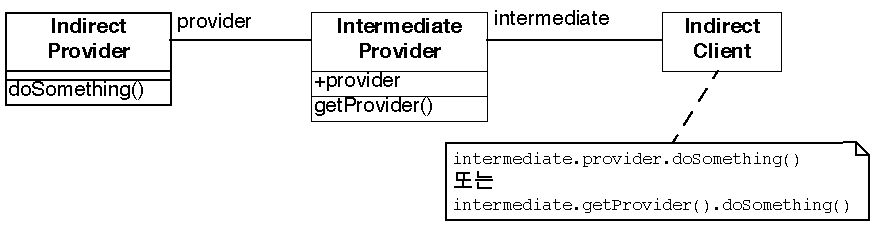
\includegraphics[width=\textwidth]{oldRedistributeDemeter.pdf}
\caption{간접 클라이언트가 중간 공급자를 통해 간접 공급자로 이동하여 두 공급자를 불필요하게 결합함으로써 \ind{디미터의 법칙}을 위반한다.}
\figlabel{RedistributeDemeter}
\end{center}
\end{figure}

\index{신 클래스}
\index{데이터 컨테이너}
데이터 컨테이너는 책임이 너무 적은 반면, 신 클래스는 너무 많은 책임을 맡는다. 신 클래스는 수천 줄의 코드와 수백 개의 메서드 및 인스턴스 변수로 구성된 전체 하위 시스템을 구현하는 단일 클래스일 수 있다. 특히 악의적인 신 클래스는 정적 인스턴스 변수와 메서드로만 구성되며, 즉 모든 데이터와 동작이 클래스 범위를 가지며, 신 클래스는 인스턴스화되지 않는다. 이러한 신 클래스는 순전히 괴물과 같은 프로시저에 불과하며 이름만 객체 지향적이다. 

때때로 \emph{유틸리티 클래스(utility class)}로 알려진 일부 프로시저 클래스가 편리하기도 하다. 가장 잘 알려진 예는 수학 라이브러리에 대한 객체 지향 인터페이스나 알고리즘 모음이다. 그러나 실제 신 클래스는 라이브러리가 아니라 전체 애플리케이션 실행을 제어하는 완전한 애플리케이션 또는 하위 시스템이다.

신 클래스와 데이터 컨테이너는 종종 함께 존재하며, 신 클래스가 애플리케이션의 모든 제어를 맡고 다른 클래스는 영광스러운 데이터 구조로 취급한다. 신 클래스는 너무 많은 책임을 맡기 때문에 이해하고 유지하기가 어렵다. 인터페이스의 복잡성과 명확한 서브클래싱 계약의 부재로 인해 상속을 통한 신 클래스의 점진적 수정 및 확장은 거의 불가능에 가깝다.

\begin{figure}[h]
\begin{center}
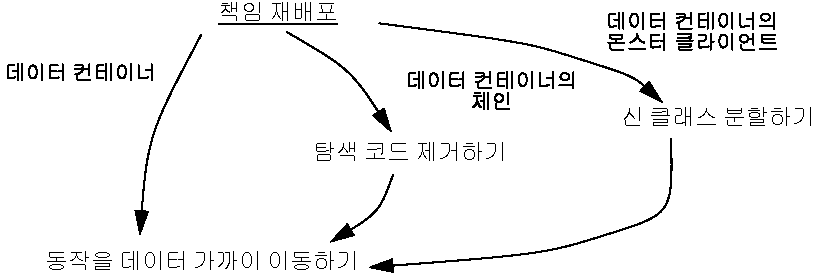
\includegraphics[width=\textwidth]{oldRedistributeMap.pdf}
\caption{데이터 컨테이너는 잘못 배치된 책임의 가장 명확한 신호이다. 이 세 가지 패턴은 동작을 데이터에 가깝게 이동하여 책임을 재분배한다.}
\figlabel{RedistributeMap}
\end{center}
\end{figure}

이 클러스터는 책임을 재분배하여 데이터 컨테이너와 신 클래스를 제거함으로써 캡슐화를 개선하는 여러 패턴을 제공한다.

\begin{bulletlist}
\item \patpgref{동작을 데이터 가까이 이동하기}{MoveBehaviorCloseToData}는 간접 클라이언트에 정의된 동작을 중간 데이터 컨테이너로 이동하여 보다 ``객체처럼'' 만든다. 이 패턴은 간접 클라이언트를 데이터 컨테이너의 콘텐츠에서 분리할 뿐만 아니라 일반적으로 데이터 컨테이너의 여러 클라이언트에서 발생하는 중복된 코드를 제거한다.

\item \patpgref{탐색 코드 제거하기}{EliminateNavigationCode}는 리엔지니어링 단계 측면에서 \patref{동작을 데이터 가까이 이동하기}{MoveBehaviorCloseToData}과 기술적으로 매우 유사하지만 그 의도는 다소 다르다. 이 패턴은 탐색 코드를 제거하기 위해 데이터 컨테이너 체인 아래로 책임을 재분배하는 데 중점을 둔다.
	
\item \patpgref{신 클래스 분할하기}{SplitUpGodClass}는 모든 데이터를 외부 데이터 컨테이너로 이동하고, 데이터 컨테이너를 객체로 승격하기 위해 \patref{동작을 데이터 가까이 이동하기}{MoveBehaviorCloseToData}를 적용하고, 마지막으로 남아 있는 파사드를 제거함으로써 프로시저 신 클래스를 더 단순하고 응집도 높은 여러 클래스로 리팩터링한다.
\end{bulletlist}

%=================================================================
%:PATTERN -- {Move Behavior Close to Data}
\pattern{동작을 데이터 가까이 이동하기}{MoveBehaviorCloseToData}

\intent{간접 클라이언트의 동작(behavior)을 동작이 처리하는 데이터가 포함된 클래스로 이동하여 캡슐화를 강화한다.}

\subsection*{문제}

클래스를 단순한 데이터 컨테이너에서 실제 서비스 프로바이더로 전환하려면 어떻게 해야 할까?

\emph{이 문제는 다음과 같은 이유로 어렵다.}

\begin{bulletlist}
\item 데이터 컨테이너는 실제 동작이 아닌 접근자 메서드(access method)나 퍼블릭 인스턴스 변수(public instance variable)만 제공하므로 클라이언트가 동작을 사용하는 대신 직접 동작을 정의해야 한다. 새 클라이언트는 일반적으로 이 동작을 다시 구현해야 한다.

\item 데이터 컨테이너의 내부 표현이 변경되면 많은 클라이언트를 업데이트해야 한다.
	
\item 데이터 컨테이너는 동작을 정의하지 않고 인터페이스가 주로 접근자 메서드로 구성되어 있기 때문에 다형성으로 사용할 수 없다. 따라서 클라이언트는 주어진 컨텍스트에서 어떤 동작이 필요한지 결정할 책임이 있다.
\end{bulletlist}

\emph{그러나 이 문제를 해결할 수 있는 이유는 다음과 같다.} 

\begin{bulletlist}
\item 클라이언트가 데이터로 어떤 작업을 수행하는지 알고 있다.
\end{bulletlist}

\subsection*{해결}

간접 클라이언트에 의해 정의된 동작을 해당 동작이 수행되는 데이터의 컨테이너로 이동한다.

\subsubsection*{탐지}

다음 사항들을 찾는다.

\begin{bulletlist}
\item 데이터 컨테이너, 즉 대부분 퍼블릭 접근자 메서드와 몇 가지 동작 메서드를 정의하는 클래스(즉, 메서드 수가 속성 수보다 약 2배 더 많음).

\item 별도의 공급자 클래스의 데이터를 조작하는 중복된 클라이언트 코드. 여러 클라이언트가 \emph{다른} 동작을 구현하는 경우, 대신 \patpgref{클라이언트 타입 검사 변환하기}{TransformClientTypeChecks}를 적용하는 것을 고려하자.

\item 클라이언트 클래스에서 일련의 접근자 메서드를 호출하는 메서드(\patref{탐색 코드 제거하기}{EliminateNavigationCode} 참조).
\end{bulletlist}

\subsubsection*{단계}

\patref{동작을 데이터 가까이 이동하기}{MoveBehaviorCloseToData}는 \patpgref{Extract 메서드 추출하기}{ExtractMethod} 및 \patpgref{메서드 이동하기}{MoveMethod}를 사용하여 리팩터링한다. 문제의 동작을 클라이언트 메서드에서 추출한 다음 프로바이더 클래스로 이동해야 하기 때문이다.

\begin{figure}
\begin{center}
\includegraphics[width=\textwidth]{RedistributeDataContainers}
\caption{단순 데이터 컨테이너에 불과했던 클래스가 실제 서비스 프로바이더로 전환된다}
\figlabel{RedistributeDataContainers}
\end{center}
\end{figure}

\begin{enumerate}
\item \emph{이동하려는 클라이언트 동작을 식별한다}, 즉 전체 메서드 또는 프로바이더 데이터에 액세스하는 메서드의 일부이다.

	\begin{bulletlist}
	\item 데이터 컨테이너의 접근자 메서드 호출을 찾는다.

	\item 동일한 프로바이더 데이터에 액세스하는 여러 클라이언트에서 중복된 코드를 찾는다.
	\end{bulletlist}

\item 프로바이더 클래스에 해당 메서드가 없는 경우\emph{프로바이더 클래스에 해당 메서드를 생성한다}. 코드를 이동해도 이름 충돌이 발생하지 않는지 확인하자. 리팩터링 브라우저 \cite{Robe97a}와 같은 도구는 이러한 단계를 자동화한다.

	\begin{bulletlist}
	\item 추출된 기능이 인수가 있는 완전한 메서드인 경우 인수가 프로바이더 클래스의 속성과 충돌하지 않는지 확인한다. 충돌하는 경우 인수의 이름을 바꾼다.  

	\item 추출된 함수가 임시 변수를 사용하는 경우 로컬 변수가 대상 범위의 속성 또는 변수와 충돌하지 않는지 확인합니다. 충돌하는 경우 임시 변수의 이름을 바꾼다.

	\item 추출된 함수가 클라이언트 클래스의 로컬 변수(속성, 임시 변수...)에 액세스하는지 확인하고, 그렇다면 이러한 클라이언트 변수를 나타내는 메서드에 인자를 추가한다. 
	\end{bulletlist}

\item \emph{새 메서드에 의도가 드러나는 이름을 지정한다.} 무엇보다도 의도를 드러내기 이름에는 메서드가 속한 클래스에 대한 참조가 포함되지 않으므로 메서드의 재사용성이 떨어진다. 예를 들어, \lct{Set} 클래스에 \lct{addToSet()} 메서드를 정의하는 대신 단순히 \lct{add()}로 이름을 지정하는 것이 좋다. 마찬가지로, 메서드 이름에는 정렬된 랜덤 액세스 컬렉션을 암시하는 반면 \lct{search()}라는 이름에는 그러한 의미가 없으므로 \lct{binarySearch()} 메서드를 \lct{Array} 클래스에 정의하는 것은 좋은 생각이 아니다.

\item 클라이언트에서 올바른 매개변수를 사용하여\emph{새 프로바이더 메서드를 호출}한다.

\item \emph{클라이언트 코드를 정리한다.} 이동된 기능이 클라이언트 클래스의 완전한 메서드인 경우.

	\begin{bulletlist}
	\item 이전 메서드를 호출하는 모든 메서드를 검사하고 이제 새 프로바이더 메서드를 대신 호출하는지 확인한다.

	\item 클라이언트에서 이전 메서드를 제거하거나 지원 중단한다. (\patpgref{폐기된 인터페이스 지원 중단하기}{DeprecateObsoleteInterfaces}).  
\end{bulletlist}

동일한 객체에 정의된 호출 메서드도 프로바이더로 이동해야 하는 경우가 있을 수 있다. 이러한 경우 메서드를 위한 단계를 반복한다.

\item 여러 클라이언트에 대해 \emph{반복}한다. 이미 프로바이더로 전송된 코드를 이동할 필요가 없으므로 여러 클라이언트에서 중복된 코드는 2단계에서 제거된다. 프로바이더에 동일하지는 않지만 유사한 메소드가 많이 도입된 경우 중복된 조각을 보호된 헬퍼 메소드로 간주하는 것이 좋다.

\end{enumerate}

\subsection*{트레이드오프}

\subsubsection*{장점}

\begin{bulletlist}
\item 데이터 컨테이너가 명확한 책임이 있는 서비스 프로바이더로 전환된다.

\item 서비스 프로바이더는 다른 클라이언트에게 더 유용해진다.

\item 클라이언트는 더 이상 프로바이더 동작을 구현할 책임이 없다.

\item 클라이언트는 프로바이더의 내부 변경에 덜 민감하다. 

\item 시스템 내 코드 중복이 감소한다.
\end{bulletlist}

\subsubsection*{단점}

\begin{bulletlist}
\item 이동된 동작이 클라이언트 데이터에도 액세스하는 경우 이러한 액세스를 매개변수로 전환하면 프로바이더의 인터페이스가 더 복잡해지고 프로바이더에서 클라이언트로의 명시적 종속성이 도입된다.
\end{bulletlist}

\subsubsection*{어려움}

\begin{bulletlist}
\item 클라이언트 코드를 실제로 데이터 프로바이더로 옮겨야 하는지 여부가 명확하지 않을 수 있다. lct{Stream} 또는 \lct{Set}과 같은 일부 클래스는 실제로 데이터 프로바이더로 설계되었다. 다음과 같은 경우 코드를 프로바이더로 옮기는 것을 고려하자.

\begin{bulletlist}
\item 기능(functionality)은 프로바이더의 \emph{책임}을 나타낸다. 예를 들어 클래스 Set은 합집합과 교집합과 같은 수학적 연산을 제공해야 한다. 반면에 일반 \lct{Set}은 \lct{Employees} 집합에 대한 연산을 담당해서는 안 된다.
\item 함수는 프로바이더의 속성에 액세스한다,
\item 기능이 여러 클라이언트에 의해 정의된다.
\end{bulletlist}

\item 프로바이더가 실제로 데이터 컨테이너로 설계된 경우 데이터 프로바이더의 인스턴스를 래핑하고 관련 동작을 보유하는 새 프로바이더 클래스를 정의하는 것을 고려하자. 예를 들어, \lct{EmployeeSet}은 \lct{Set} 인스턴스를 래핑하고 더 적합한 인터페이스를 제공할 수 있다.
\end{bulletlist}

\subsubsection*{레거시 솔루션이 최종 솔루션인 경우}

데이터 컨테이너는 기존 데이터베이스에 객체 인터페이스를 제공하기 위해 데이터베이스 스키마에서 자동으로 생성되었을 수 있다. 코드를 다시 생성해야 하는 경우 변경 사항을 잃게 되므로 생성된 클래스를 수정하는 것은 거의 항상 좋지 않은 생각이다. 이 경우 래퍼 클래스를 구현하여 생성된 클래스와 연관되어야 하는 동작을 보유할 수 있다. 이러한 래퍼는 생성된 데이터 컨테이너를 실제 서비스 프로바이더로 변환하는 \patpgref{어댑터}{Adapter}로 작동한다. 

라이브러리에 정의된 클래스에 중요한 기능이 누락되어 있는 경우가 있다. 예를 들어, \lct{String} 클래스에 \lct{convertToCapitals} 연산이 누락되어 있는 경우를 들 수 있다. 이러한 경우 일반적으로 라이브러리에 코드를 추가하는 것이 불가능하므로 클라이언트 클래스에서 정의해야 할 수 있다. 예를 들어 \ind{C++}에서는 코드를 사용할 수 없을 때 재컴파일을 피하거나 클래스를 확장하는 유일한 방법일 수 있다 \cite{Alpe98a} (378페이지). \ind{Smalltalk}에서는 라이브러리를 확장하거나 수정할 수 있지만, 추가 코드를 분리하여 향후 라이브러리 릴리스와 쉽게 병합하고 충돌을 빠르게 감지할 수 있도록 각별히 주의해야 한다. 

\patpgref{비지터}{Visitor} 디자인 패턴의 의도는 다음과 같다: \emph{``객체 구조의 요소에 대해 수행할 연산을 요소 자체와는 별도로 클래스에 표시한다. \patref{비지터}{Visitor}를 사용하면 연산이 수행되는 요소의 클래스를 변경하지 않고도 새로운 연산을 정의할 수 있다.'' } \cite{Gamm95a}. \patref{비지터}{Visitor} 패턴은 클래스가 별도의 프로바이더 클래스의 데이터에 액세스하도록 하려는 몇 안 되는 경우 중 하나이다. \patref{비지터}{Visitor}를 사용하면 안정된 클래스 집합을 변경하지 않고도 새 연산을 동적으로 추가할 수 있다. 

\emph{구성 클래스(configuraton class)}는 시스템의 구성을 나타내는 클래스이다(예: 전역 매개변수, 언어에 따른 표현, 적용 중인 정책). 예를 들어 그래픽 도구에서 상자의 기본 크기, 가장자리, 선의 너비 등을 이러한 클래스에 저장하고 필요할 때 다른 클래스가 이를 참조할 수 있다. 

\emph{매핑 클래스(mapping class)}는 객체와 객체의 사용자 인터페이스 또는 데이터베이스 표현 간의 매핑을 나타내는 데 사용되는 클래스이다. 예를 들어, 소프트웨어 지표 도구는 사용자가 계산할 지표를 선택할 수 있도록 위젯 목록에서 사용 가능한 지표를 그래픽으로 표현해야 한다. 이러한 경우 서로 다른 메트릭의 그래픽 표현은 내부 표현과 분명히 다를 것이다. 매핑 클래스는 연관성을 추적한다.

\subsection*{예시}

고객들의 반복되는 불만 중 하나는 정보 시스템에서 생성된 보고서를 변경하는 데 너무 많은 시간이 걸린다는 것이다. 유지 관리자와 이야기를 나누다 보면 보고서 생성이 매우 지루하다는 것을 알게 된다. ``항상 똑같은 코드를 작성해야 해요.''라고 유지관리자인 크리스가 말한다. ``데이터베이스에서 레코드를 가져와서 해당 필드를 인쇄한 다음 다음 레코드로 넘어가면 되요.'' 

데이터 컨테이너의 경우를 강력하게 의심하고 코드를 자세히 살펴보면 의심을 확인할 수 있다. 데이터베이스와 인터페이스하는 거의 모든 클래스에는 접근자 메서드만 포함되어 있으며, 보고서를 생성하는 프로그램에서는 이러한 접근자를 사용할 수밖에 없다. 한 가지 눈에 띄는 예는 \lct{Payroll} 애플리케이션의 경우로, \lct{TelephoneGuide} 애플리케이션과 공통점이 많아서 공통 기능을 \lct{Employee} 클래스로 옮기기로 결정한 경우이다.

\subsubsection*{예전}

\begin{figure}
\begin{center}
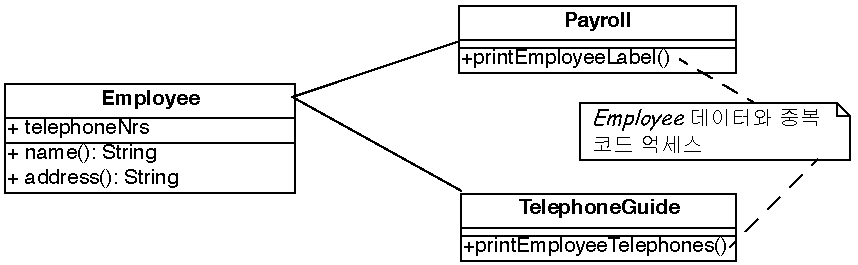
\includegraphics[width=\textwidth]{oldRedistributeBefore.pdf}
\caption{\lct{Payroll} 및 \lct{Telephone} 클래스는 \lct{Employee} 클래스의 내부 표현에 액세스하여 표현(representation)을 인쇄한다.}
\figlabel{RedistributeBefore}
\end{center}
\end{figure}

\figref{RedistributeBefore}에 표시된 것처럼 \lct{Payroll} 및 \lct{TelephoneGuide} 클래스는 모두 \lct{Employee} 인스턴스를 데이터 컨테이너로 취급하여 레이블을 인쇄한다. 따라서 \lct{Payroll}과 \lct{TelephoneGuide}는 \lct{Employee} 속성의 간접 클라이언트이며, \lct{Employee} 클래스에서 제공해야 하는 인쇄 코드를 정의한다. 다음 코드는 \ind{Java}에서 어떻게 표시되는지 보여준다.

\begin{code}
public class Employee {
	public String[] telephoneNumbers = {};
	...
	public String name() {
		return name;}
	
	public String address() {
		return address;}
}

public class Payroll {

	public static Employee currentEmployee;

	public static void printEmployeeLabel () {
		System.out.println(currentEmployee.name());
		System.out.println(currentEmployee.address());
		for (int i=0; i < currentEmployee.telephoneNumbers.length; i++) {
			System.out.print(currentEmployee.telephoneNumbers[i]);
			System.out.print(" ");}
		System.out.println("");}
...
}

public class TelephoneGuide {

	public static void printEmployeeTelephones (Employee emp) {
		System.out.println(emp.name());
		System.out.println(emp.address());
		for (int i=0; i < emp.telephoneNumbers.length - 1; i++) {
			System.out.print(emp.telephoneNumbers[i]);
			System.out.print(" -- ");}
		System.out.print(emp.telephoneNumbers[
				emp.telephoneNumbers.length - 1]);
		System.out.println("");}
	...
}
\end{code}

두 인쇄 메서드는 본질적으로 동일한 기능을 구현하지만 약간의 차이점이 있다. 그 중에서도 \lct{TelephoneGuide.printEmployeeTelephones}는 전화번호를 인쇄할 때 다른 구분 기호를 사용한다.

\subsubsection*{단계}

사용할 구분 기호를 나타내는 특수 매개 변수를 정의하여 다른 구분 기호를 쉽게 처리할 수 있다. 따라서 \lct{TelephoneGuide.printEmployeeTelephones}는 다음과 같이 재작성된다.

\begin{code}
	public static void printEmployeeTelephones
						(Employee emp, String separator) {
		...
		for (int i=0; ...
			System.out.print(separator);}
		...}
	...
\end{code}

다음으로, \lct{printEmployeeTelephones} 메서드를 \lct{TelephoneGuide}에서 \lct{Employee}로 옮긴다. 따라서 코드를 복사하고 \lct{emp} 매개 변수에 대한 모든 참조를 속성 및 메서드에 대한 직접 참조로 바꾼다. 또한 새 메서드에 의도를 드러내는 이름이 있는지 확인하여 메서드 이름에서 \lct{Employee} 부분을 생략하여 \lct{printLabel}이라는 메서드를 생성한다.

\begin{code}
public class Employee {
	...
	public void printLabel (String separator) {
		
		System.out.println(name);
		System.out.println(address);
		for (int i=0; i < telephoneNumbers.length - 1; i++) {
			System.out.print(telephoneNumbers[i]);
			System.out.print(separator);
		}
		System.out.print(telephoneNumbers[telephoneNumbers.length - 1]);
		System.out.println("");
	}
\end{code}

그런 다음 \lct{Payroll.printEmployeeLabel} 및 \lct{TelephoneGuide.printEmployeeTelephones}의 메서드 본문을 \lct{Employee.printLabel} 메서드의 간단한 호출로 대체한다.

\begin{code}
public class Payroll {
	...
	public static void printEmployeeLabel () {
		currentEmployee.printLabel(" ");
	...}

public class TelephoneGuide {
	...
	public static void printEmployeeTelephones (Employee emp) {
		emp.printLabel(" -- ");}
	...}
\end{code}

마지막으로 어떤 다른 메서드가 \lct{name()}, \lct{address()} 및 \lct{전화번호}를 참조하는지 확인한다. 이러한 메서드가 존재하지 않는다면 해당 메서드와 속성을 \lct{private}로 선언하는 것이 좋다.

\subsubsection*{이후}

\patref{동작을 데이터 가까이 이동하기}{MoveBehaviorCloseToData}를 적용한 후 \lct{Employee} 클래스는 이제 하나의 인수를 받아 다른 구분 기호를 나타내는 \lct{printLabel} 메서드를 제공한다(\figref{RedistributeAfter} 참조). 이제 클라이언트가 \lct{Employee}의 내부 표현에 의존하지 않기 때문에 더 나은 상황이다. 또한 동작을 작동하는 데이터 근처로 이동시킴으로써 클래스는 구현하는 구조 대신 프로바이더가 제공하는 서비스에 중점을 둔 개념적 엔티티를 나타낸다.

\begin{figure}
\begin{center}
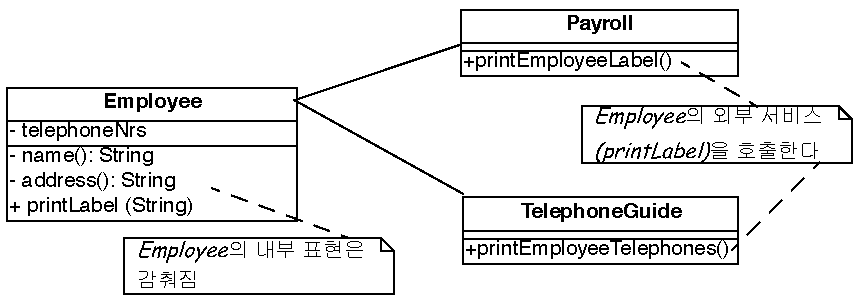
\includegraphics[width=\textwidth]{oldRedistributeAfter.pdf}
\caption{\lct{Payroll} 클래스는 \lct{Employee} 클래스의 퍼블릭 인터페이스를 사용하여 \lct{Employee}의 표현을 인쇄하며, 데이터 액세서는 비공개가 되었다.}
\figlabel{RedistributeAfter}
\end{center}
\end{figure}


\subsection*{근거}

\index{리엘, 아서}
\begin{quotation}
\emph{관련 데이터와 동작을 한 곳에 보관하자.}

\hfill  --- 아서 리엘, 휴리스틱 2.9 \cite{Riel96a}
\end{quotation}

데이터 컨테이너는 구조를 노출하고 클라이언트가 동작을 공유하기보다는 정의하도록 강요하기 때문에 진화를 저해한다. 서비스 프로바이더에게 데이터 컨테이너를 장려하면 클래스 간의 결합도를 줄이고 데이터와 동작의 응집도를 향상시킬 수 있다.

\subsection*{관련 패턴}

\patpgref{필드 캡슐화하기}{EncapsulateField}는 설계 단계에서 메서드를 정의해야 하는 위치를 결정하는 데 도움이 되는 휴리스틱을 제공한다. 이 텍스트는 \patref{동작을 데이터 가까이 이동하기}{MoveBehaviorCloseToData}를 적용하기 위한 근거를 제공한다.

%=================================================================
%:PATTERN -- {Eliminate Navigation Code}
\pattern{탐색 코드 제거하기}{EliminateNavigationCode}

\ind{디미터의 법칙} \cite{Lieb88a}으로도 알려져 있다

\intent{연결된 클래스 체인으로 책임을 전가하여 변경의 영향을 줄인다.}

\subsection*{문제}

객체 그래프를 탐색하는 클래스로 인한 결합도를 줄이려면 어떻게 해야 할까?

\emph{이 문제는 다음과 같은 이유로 어렵다.} 

\begin{bulletlist}
\item 클래스의 인터페이스 변경은 직접 클라이언트뿐만 아니라 해당 클래스에 도달하기 위해 탐색하는 모든 간접 클라이언트에도 영향을 미친다.
\end{bulletlist}

\emph{그러나 이 문제를 해결할 수 있는 이유는 다음과 같다.}

\begin{bulletlist}
\item 탐색 코드는 일반적으로 잘못 배치된 책임과 캡슐화 \subind{캡슐화}{위반}의 신호이다.
\end{bulletlist}

\subsection*{해결}

간접 클라이언트에 의해 정의된 동작을 해당 동작이 작동하는 데이터 컨테이너로 반복적으로 이동한다.

실제 리엔지니어링 단계는 기본적으로 \patref{동작을 데이터 가까이 이동하기}{MoveBehaviorCloseToData}의 단계와 동일하지만 문제의 양상이 다소 다르므로 다른 탐지 단계가 적용된다는 점에 유의하자.

\subsubsection*{탐지}

\emph{간접프로바이더}를 찾는다.

\begin{bulletlist}
\item 클래스가 변경될 때마다, 예를 들어 내부 표현이나 공동 작업자를 수정하여 변경할 때마다 직접 클래스뿐만 아니라 \emph{간접} 클라이언트 클래스도 변경해야 한다.

\item 퍼블릭 속성, 접근자 메서드 또는 클래스의 값 속성(value attribute)으로 반환되는 메서드가 많이 포함된 클래스를 찾는다.

\item 대부분 데이터 클래스를 포함하는 큰 에그리게이션 계층 구조는 종종 간접 프로바이더 역할을 한다.
\end{bulletlist}

\emph{탐색 코드(navigation code)}가 많이 포함된 \emph{간접 클라이언트}를 찾는다. 탐색 코드는 두 가지 종류가 있다.

\begin{bulletlist}
\item \emph{속성 액세스 시퀀스(sequence of attribute accesses)}, \eg \lct{a.b.c.d} 여기서 b는 a의 속성, c는 b의 속성, d는 c의 속성이다. 이러한 시퀀스의 결과는 변수에 할당되거나 마지막 객체의 메서드가 호출될 수 있으며, \eg \lct{a.b.c.d.op()}이 될 수 있다. 이러한 시퀀스 탐색은 모든 어트리뷰트가 보호되는 Smalltalk에서는 발생하지 않는다. 

\item \emph{접근자 메서드 호출의 시퀀스(sequence of accessor method calls)}. Java와 C++에서 이러한 시퀀스는 \lct{object.m1().m2().m3()}의 형태를 갖는다. 여기서 \lct{object}는 객체를 반환하는 표현식, \lct{m1}은 \lct{object}의 메서드, \lct{m2}는 \lct{m1}의 호출로 반환된 객체의 메서드, \lct{m2}의 호출로 반환된 객체의 메서드 등등이 있다. Smalltalk에서 탐색 코드는 다음과 같은 형식의 리시버 \lct{m1 m2 ... mn}을 갖는다. 동일한 탐색 코드 시퀀스는 동일하거나 다른 클라이언트에서 다른 메서드에서 반복된다.
\end{bulletlist}

탐색 코드는 간단한 패턴 매칭으로 감지할 수 있다. 그러나 실제로 결합된 클래스로 이어지는 메서드 호출 탐색 시퀀스를 탐지하려면 한 객체를 다른 객체로 변환하는 호출 시퀀스를 필터링해야 한다. 예를 들어, 다음 두 Java 표현식은 객체 변환을 다루기 때문에 문제가 되지 않는다.

\begin{code}
leftSide().toString()
i.getValue().isShort()
\end{code}

이 경우를 처리하려면 다음과 같이 하면 된다.

\begin{bulletlist}
\item 두 개 이상의 호출을 찾기. 또는 

\item 원시 타입으로 변환하거나 원시 타입에서 변환하기 위한 표준 메서드 호출을 포함하여 알려진 객체 변환 호출을 고려 대상에서 제거하기.
\end{bulletlist}

추가 변수를 사용하면 탐색 코드를 위장할 수 있으므로 코드를 읽어야 하는 경우가 종종 있다. 예를 들어 다음 Java 코드에는 호출 체인이 포함되어 있지 않다.

\begin{code}
Token token;
token = parseTree.token();
if (token.identifier() != null) {
	...
\end{code}

그러나 호출 체인을 포함하는 다음 코드와 동일하다.

\begin{code}
if (parseTree.token().identifier() != null) {
	...
\end{code}

\noindent
\emph{\ind{Smalltalk}.}
Smalltalk에는 미리 정의된 제어 구조체가 없고 제어 구조체를 구현할 때도 메시지를 사용하기 때문에 Smalltalk 코드에서 단순히 호출 시퀀스를 검색하는 것은 많은 노이즈를 생성할 수 있다. 위장된 탐색 코드가 있는 위의 예제는 Smalltalk에서 다음과 같이 읽힐 것이다. (\lct{isNil}과 \lct{ifFalse:[...]} 메시지에 주목하자).

\begin{code}
| token |
token := parseTree token.
token identifier isNil ifFalse:[...]
\end{code}

탐색 코드와 동등한 버전이 된다.

\begin{code}
parseTree token identifier isNil ifFalse: [...]
\end{code}

다음 코드 세그먼트에는 일련의 호출이 포함되어 있지만 첫 번째는 부울 테스트를 다루고 두 번째는 변환(사실 변환 남용)을 다루기 때문에 문제가 되지 않는다.

\begin{code}
(a isNode) & (a isAbstract) ifTrue: [...]
aCol asSet asSortedCollection asOrderedCollection 
\end{code}

\noindent
\emph{\ind{Java}.}
Java 또는 C++의 경우, 기본 데이터 타입과 제어 구조는 객체를 사용하여 구현되지 않으므로 간단한 패턴 일치는 노이즈가 적다. 예를 들어, 다음과 같은 간단한 Unix 명령은 노이즈가 적다.

\begin{code}
egrep '.*\(\).*\(\).*\(\).' *.java
egrep '.*\..*\..*\..' *.java
\end{code}
\noindent
클래스 간 탐색 코드 결합도의 예인 다음과 같은 코드 줄을 식별하고 위에서 언급한 변환을 필터링한다. 


\begin{code}
a.getAbstraction().getIdentifier().traverse(this) 
a.abstraction.identifier.traverse(this)
\end{code}

보다 정교한 매칭 표현식을 사용하면 대괄호 또는 다른 조합의 괄호로 인해 발생하는 노이즈를 줄일 수 있다.

\noindent
\emph{\ind{AST 매칭}.}
트리 매칭을 표현하는 방법이 있는 경우 탐색 코드를 감지할 수 있다. 예를 들어, \ind{리팩토링 브라우저}(Refactoring Browser)와 함께 제공되는 \ind{다시 쓰기 규칙 편집기}(Rewrite Rule Editor)는 다음과 같다. \cite{Robe97a}는 \lct{'@object 'mess1 'mess2 'mess3} 패턴을 사용하여 탐색 코드를 감지할 수 있다. 결과 분석 범위를 좁히려면 도메인 객체에 속하는 메시지만 고려하고 라이브러리 객체의 메서드 선택자(예: \lct{isNil}, \lct{not}, \lct{class}, ...)를 모두 제거해야 한다.

\subsubsection*{단계}

\begin{figure}
\begin{center}
\includegraphics[width=0.8\textwidth]{RedistributeChains}
\caption{데이터 컨테이너 체인을 서비스 프로바이더로 변환하여 탐색 코드를 없애고 클래스 간 결합도를 줄일 수 있다.}
\figlabel{RedistributeChains}
\end{center}
\end{figure}

탐색 코드를 제거하는 방법은 재귀적으로 \patref{동작을 데이터 가까이 이동하기}{MoveBehaviorCloseToData}를 사용하는 것이다. \figref{RedistributeChains}은 이 변환을 보여준다.
\begin{enumerate}
\item 이동할 탐색 코드 \emph{구별하기(Identify)}
\item \patref{동작을 데이터 가까이 이동하기}{MoveBehaviorCloseToData}를 사용하여 탐색의 한 수준을 제거하기를 \emph{적용하기(Apply)}. (이 시점에서 회귀 테스트가 실행되어야 한다.)
\item 필요한 경우 \emph{반복(Repeat)}하기
\end{enumerate}

\noindent
\emph{주의.}
리팩터링 프로세스는 \emph{클라이언트에서 프로바이더로} 코드를 푸시하는 것에 의존한다는 점에 유의하는 것이 중요하다. 이 예에서는 \lct{Car}에서 \lct{Engine}으로, \lct{Engine}에서 \lct{Carburetor}로 푸시한다. 일반적인 실수는 클라이언트 클래스 수준에서 프로바이더 속성 값의 속성에 액세스하는 접근자를 정의하여 탐색 코드를 제거하려고 하는 것이다(예: \lct{Car} 클래스에 접근자 \lct{getCarburetor}를 정의하는 것). 클래스 간의 결합도가 줄어드는 대신 퍼블릭 접근자의 수가 증가하고 시스템이 더 복잡해진다.

\subsection*{트레이드오프}

\subsubsection*{장점}

\begin{bulletlist}
\item 클래스 간의 종속성 사슬이 제거되어 최하위 레벨의 클래스 변경이 더 적은 수의 클라이언트에 영향을 미친다.

\item 시스템에 암시되어 있던 기능이 이제 새 클라이언트에서 이름을 지정하고 명시적으로 사용할 수 있다.
\end{bulletlist}

\subsubsection*{단점}

\begin{bulletlist}
\item \patref{탐색 코드 제거하기}{EliminateNavigationCode}를 체계적으로 적용하면 인터페이스가 커질 수 있다. 특히 클래스가 컬렉션인 인스턴스 변수를 많이 정의하는 경우 \patref{탐색 코드 제거하기}{EliminateNavigationCode}를 사용하면 기본 컬렉션을 보호하기 위해 많은 수의 추가 메서드를 정의해야 할 수 있다. 
\end{bulletlist}

\subsubsection*{어려움}

\begin{bulletlist}
\item \patref{탐색 코드 제거하기}{EliminateNavigationCode}를 언제 적용할지 결정하는 것은 어려울 수 있다. 단순히 클래스 공동 작업자에게 요청을 위임하는 메서드를 정의하는 것이 항상 해결책이 될 수는 없다. 내부 정보를 제공하면 클래스의 인터페이스가 축소될 수 있다. 예를 들어 클래스가 잘 정의된 몇 가지 동작을 구현하지만 다른 공동 작업자에게 \patpgref{파사드}{Facade} 역할을 하는 경우, 클래스의 인터페이스를 줄이기 위해 공동 작업자에게 직접 액세스 권한을 부여하는 것이 더 간단할 수 있다.
\end{bulletlist}

\subsubsection*{레거시 솔루션이 최종 솔루션인 경우}

객체가 그래픽으로 표시되거나 데이터베이스에 매핑되는 경우 탐색 코드가 최상의 솔루션일 수 있다. 이러한 경우 목표는 클래스 간의 구조적 관계를 실제로 노출하고 모방하는 것이다. 내비게이션 코드를 제거하는 것은 쓸데없는 일이 될 것이다. 

클라이언트가 간접 프로바이더와 대화해야 하는 경우도 있다. 직접 프로바이더가 특정 속성(OOID, 키...)이 주어진 특정 객체를 반환하는 객체 서버 역할을 하는 경우가 이에 해당한다. 이 경우 클라이언트는 클라이언트가 메시지를 보내는 객체(간접 프로바이더)를 반환하는 객체 \emph{서버}(직접 프로바이더)를 호출한다. 

\subsection*{예시}

\lct{Employee}, \lct{Payroll}, \lct{TelephoneGuide} 클래스를 수정한 후 전체 프로젝트를 다시 빌드하는 데 30분이 걸렸다는 것을 알 수 있다. 다음에 크리스(유지관리자 중 한 명)를 만나면 왜 이렇게 오래 걸렸냐고 물어보자. ``아마 Employee 클래스를 변경하셨을 거에요.'' 그는 ``많은 클래스가 그 클래스에 의존하기 때문에 감히 그 클래스를 건드리지 못했어요.''라고 대답한다.

\begin{figure}
\begin{center}
\includegraphics[width=0.8\textwidth]{RedistributeDependencies}
\caption{\lct{Reports} 클래스와 \lct{File} 및 \lct{Employee} 클래스 간의 불필요한 종속성을 제거하는 방법.}
\figlabel{RedistributeDependencies}
\end{center}
\end{figure}

이 \lct{Employee} 클래스를 더 자세히 살펴보고 불필요한 종속성을 많이 찾기로 결정한다. 예를 들어 (\figref{RedistributeDependencies}에 표시된 것처럼) 모든 \lct{employees}이 처리하는 파일 수를 각 \lct{Department}에 대해 계산하는 \lct{countHandledFiles} 메서드 하나를 구현하는 \lct{Reports} 클래스가 있다. 안타깝게도 \lct{Department}와 \lct{File} 사이에는 직접적인 관계가 없으므로 \lct{ReportHandledFiles}는 모든 \lct{files}을 열거하고 \lct{handled()} 상태에 액세스하기 위해 부서의 \lct{employees}를 탐색해야 한다.

아래의 \ind{Java} 코드는 \patref{탐색 코드 제거하기}{EliminateNavigationCode}를 적용하기 전과 후의 상황을 보여준다. 굵은 텍스트 요소는 적용 전후 상황의 문제와 해결 방법을 강조한다.

\subsubsection*{예전}

\begin{code}
public class Reports {
...
	public static void countHandledFiles(Department department) {
		int nrHandled = 0, nrUnhandled = 0;
	
		for (int i=0; i < department.employees.length; i++) {
			for (int j=0; j < department.employees[i].files.length; j++) {
				if (department.employees[i].files[j].handled()) {
					nrHandled++;}
				else {
					nrUnhandled++;}}}
...}
\end{code}

\lct{countHandledFiles} 메서드는 현재 부서의 \lct{employees}과 각 \lct{files}을 요청하여 처리된 파일 수를 계산한다. lct{Department} 및 \lct{Employee} 클래스는 이러한 속성을 공개로 선언해야 한다. 이 구현에서는 두 가지 문제가 발생한다. 
\begin{enumerate}
  \item \lct{Reports} 클래스는 \lct{Department}, \lct{Employee} 및 \lct{File} 간의 연결을 열거하는 방법을 알고 있어야 하며, 이 정보는 각 클래스의 퍼블릭 인터페이스에서 액세스할 수 있어야 한다. 이러한 퍼블릭 인터페이스 중 하나가 변경되면 이 변경 사항은 관련된 모든 클래스에 영향을 미친다. 
  \item \lct{countHandledFiles} 메서드는 \lct{employees} 및 \lct{files} 변수에 직접 액세스하여 구현된다. 이렇게 하면 \lct{Reports} 클래스와 \lct{Department} 및 \lct{Employee} 클래스가 불필요하게 결합된다. lct{Department} 또는 \lct{Employee} 클래스가 연결된 객체를 골드화하는 데 사용되는 데이터 구조를 변경하면 \lct{Reports} 클래스의 모든 메서드를 조정해야 한다. 
\end{enumerate}

\subsubsection*{단계}

해결책은 중첩된 \lct{for} 루프를 별도의 메서드로 추출하여 적절한 클래스로 옮기는 것이다. 이것은 실제로 두 단계의 과정이다.

먼저 \lct{Reports.countHandledFiles}에서 외부 for 루프를 별도의 메서드로 추출하고(이름도 \lct{countHandledFiles}로 지정), 이를 \lct{Department} 클래스로 옮긴다.

\begin{code}
public class Department {
...
		public void countHandledFiles
				(Counter nrHandled, Counter nrUnhandled) {
		for (int i=0; i < this.employees.length; i++) {
			for (int j=0; j < this.employees[i].files.length; j++) {
				if (this.employees[i].files[j].handled()) {
					nrHandled.increment();}
				else {
					nrUnhandled.increment();}}}}
...}

public class Reports {
...
	private static void countHandledFiles(Department department) {
		Counter nrHandled = new Counter (0), nrUnhandled = new Counter (0);
		department.countHandledFiles(nrHandled, nrUnhandled);
...}
\end{code}

다음으로, \lct{Department.countHandledFiles}(\lct{countHandledFiles}라고도 함)에서 내부 for 루프를 추출하여 Employee 클래스로 이동한다.

\begin{code}
public class Employee {
...
	public void countHandledFiles
				(Counter nrHandled, Counter nrUnhandled) {
		for (int j=0; j < this.files.length; j++) {
			if (this.files[j].handled()) {
				nrHandled.increment();}
			else {
				nrUnhandled.increment();}}}
...}

public class Department {
...
	public void countHandledFiles
				(Counter nrHandled, Counter nrUnhandled) {
		for (int i=0; i < this.employees.length; i++) {
			this.employees[i].countHandledFiles(nrHandled, nrUnhandled);}}
...}
\end{code}

\lct{employees} 및 \lct{files} 변수에 대한 모든 직접 액세스를 제거하면 이러한 속성을 프라이빗(private)으로 선언할 수 있다. 

\subsection*{예시}

\begin{quotation}
\noindent
\emph{객체 ``O''의 메서드 ``M''은 다음 종류의 객체의 메서드만 호출해야 한다.
\begin{enumerate}
  \item 자체
  \item 매개변수
  \item 이 메서드가 생성하는 모든 객체
  \item 이 메서드의 직접 컴포너트 객체
\end{enumerate}}

\hfill --- \ind{디미터 법칙}
\end{quotation}

디미터의 법칙\cite{Lieb88a}을 위반하는 탐색 코드는 잘못된 동작의 잘 알려진 증상이다 \cite{Lore94a} \cite{Shar97a} \cite{Riel96a}. 클래스 간에 불필요한 종속성이 발생하고 결과적으로 클래스의 표현을 변경하려면 \emph{모든} 클라이언트를 조정해야 한다.

\subsection*{관련 패턴}

\patref{탐색 코드 제거하기}{EliminateNavigationCode}와 \patpgref{기계적으로 코드 비교하기}{CompareCodeMechanically}는 서로를 강화한다. 여러 클라이언트에 분산되어 있는 탐색 코드는 시스템 전체에 중복된 코드를 분산시킵니다. \patref{기계적으로 코드 비교}{CompareCodeMechanically}는 이 현상을 감지하는 데 도움이 된다. \patref{탐색 코드 제거하기}{EliminateNavigationCode}는 중복된 코드를 한곳으로 모아 리팩터링하고 제거하기 쉽게 해준다.

%=================================================================
%:PATTERN -- {Split Up God Class}
\pattern{신 클래스 분할하기}{SplitUpGodClass}

\ind{더 블롭}(The Blob) \cite{Brow98a}, \ind{신 클라스}(God Class) \cite{Riel96a}로도 알려져 있다.

\intent{책임이 너무 많은 클래스를 여러 개의 작고 응집도 높은 클래스로 분할한다.}

\subsection*{문제}

너무 많은 책임을 맡은 클래스를 어떻게 유지 관리할 수 있을까?

\emph{이 문제는 다음과 같은 이유로 어렵다.} 

\begin{bulletlist}
\item 너무 많은 책임을 맡음으로써 신 클래스는 애플리케이션의 제어권을 독점하게 된다. 거의 모든 변경 사항이 이 클래스에 영향을 미치고 여러 책임에 영향을 미치기 때문에 애플리케이션의 발전이 어렵다.

\item 신 클래스에 섞여 있는 여러 추상화를 이해하기 어렵다. 여러 추상화의 데이터 대부분은 서로 다른 위치에서 액세스한다.

\item 시스템의 다른 기능이나 다른 개체에 영향을 주지 않으면서 기능을 변경할 위치를 파악하는 것은 어렵다. 또한 다른 객체의 변경은 신 클래스에 영향을 미쳐 시스템의 진화를 방해할 가능성이 높다. 

\item 신 클래스의 동작 일부를 블랙박스 방식으로 변경하는 것은 거의 불가능다.
\end{bulletlist}

\emph{그러나 이 문제를 해결할 수 있는 이유는 다음과 같다.}

\begin{bulletlist}
\item 문제를 한 번에 해결할 필요는 없습니다.

\item \ind{시맨틱 래퍼}(Semantic Wrapper)를 사용하여 래핑하고 인터페이스를 표시할 수 있다.
\end{bulletlist}

\subsection*{해결}

신 클래스의 책임을 협업하는 클래스 또는 신 클래스를 끌어낸 새 클래스에 점진적으로 재분배한다. 신 클래스에 파사드만 남으면 파사드를 제거하거나 지원 중단한다.

\subsubsection*{탐지}

신 클래스는 다양한 방식으로 인식할 수 있다.

\begin{bulletlist}
\item 하나의 거대한 클래스는 다른 많은 클래스를 데이터 구조로 취급한다.

\item ``루트'' 클래스 또는 다른 거대한 클래스는 ``System'', ``Subsystem'', ``Manager'', ``Driver'' 또는 ``Controller''와 같은 단어가 포함된 이름을 가진다.

\item 시스템에 대한 변경이 항상 동일한 클래스에 대한 변경을 초래한다.

\item 클래스에 대한 변경은 클래스의 어느 부분에 영향을 미치는지 식별할 수 없기 때문에 매우 어렵다.

\item 클래스를 재사용하는 것은 너무 많은 디자인 문제를 다루기 때문에 거의 불가능하다.

\item 해당 클래스가 시스템 또는 하위 시스템의 속성 및 메서드 대부분을 보유한 도메인 클래스이다. (일부 UI 프레임워크는 메서드가 많은 큰 클래스를 생성하고 일부 데이터베이스 인터페이스 클래스에는 많은 속성이 필요할 수 있으므로 이 임계값이 절대적인 것은 아니다.) 

\item 클래스에 분리된 인스턴스 변수에 대해 작동하는 관련 없는 메서드 집합이 있다. 클래스의 응집도가 일반적으로 낮다. 

\item 클래스가 작은 수정에도 컴파일 시간이 오래 걸린다.

\item 클래스가 많은 책임을 맡고 있어 테스트하기 어렵다.

\item 클래스가 많은 메모리를 사용한다.

\item 사람들이 말하길 ``이것이 시스템의 핵심이다''라고 말한다.

\item 신 클래스의 책임을 물어보면 다양하고 길고 불명확한 대답을 듣는다.

\item 신 클래스는 유지 관리자의 악몽이므로 어떤 클래스가 크고 유지 관리가 어려운지 물어자. 담당하고 싶지 않은 클래스가 무엇인지 물어보자. (변형: 사람들에게 작업하고 싶은 클래스를 선택하게 하자. 모두가 피하는 클래스는 신 클래스가 될 수 있다.)
\end{bulletlist}

\subsubsection*{단계}

이 솔루션은 신 클래스로부터 점진적으로 멀어지는 동작에 의존한다. 이 과정에서 데이터 컨테이너는 신 클래스가 데이터에 대해 수행하던 기능을 획득함으로써 더욱 객체와 유사해진다. 일부 새로운 클래스도 신 클래스에서 추출된다.

다음 단계에서는 이 프로세스가 이상적으로 작동하는 방식을 설명한다. 그러나 신 클래스는 내부 구조가 매우 다양할 수 있으므로 변환 단계를 구현하는 데 다른 기술을 사용할 수 있다. 또한 신 클래스는 한 번에 치료할 수 없으므로 안전한 진행 방법은 먼저 신 클래스를 가벼운 신 클래스로 변환한 다음 지인에게 동작을 위임하는 \patpgref{파사드}{Facade}로 변환하는 것이다. 마지막으로 클라이언트는 리팩터링된 데이터 컨테이너와 다른 새 객체로 리디렉션되고 \patref{파사드}{Facade}는 제거될 수 있다. 이 과정은 그림 39에 설명되어 있다.

\begin{figure}
\begin{center}
\includegraphics[width=0.8\textwidth]{RedistributeGodClass}
\caption{신 클래스는 두 단계로 리팩터링되는데, 먼저 데이터 컨테이너에 책임을 재분배하거나 새 클래스를 스폰하여 파사드만 남을 때까지 리팩터링하고 두 번째 단계는 파사드를 제거한다.}
\figlabel{RedistributeGodClass}
\end{center}
\end{figure}

다음 단계는 반복적으로 적용된다. \patpgref{변경할 때마다 회귀 테스트하기}{RegressionTestAfterEveryChange}을 적용해야 한다.
\begin{enumerate}
\item 신 클래스의 인스턴스 변수의 응집도 있는 하위 집합을 식별하고 이를 외부 데이터 컨테이너로 변환한다. 신 클래스의 초기화 메서드가 새 데이터 컨테이너의 인스턴스를 참조하도록 변경한다.

\item 신 클래스가 데이터 컨테이너로 사용하는 모든 클래스(1단계에서 생성한 클래스 포함)를 식별하고 \patref{동작을 데이터 가까이 이동하기}{MoveBehaviorCloseToData}를 적용하여 데이터 컨테이너를 서비스 프로바이더로 승격한다. 신 클래스의 원래 메서드는 단순히 이동된 메서드에 동작을 위임한다.

\item 1단계와 2단계를 반복적으로 적용하면 신 클래스에는 큰 초기화 메서드가 있는 파사드 외에는 아무것도 남지 않는다. 초기화에 대한 책임을 별도의 클래스로 이동하여 순수한 파사드만 남도록 한다. 클라이언트를 이전 신 클래스가 이제 파사드인 객체로 반복적으로 리디렉션하고 파사드를 지원 중단하거나(\patpgref{폐기된 인터페이스 지원 중단하기}{DeprecateObsoleteInterfaces} 참조) 단순히 제거다.
\end{enumerate}

\subsection*{트레이드오프}

\subsubsection*{장점}

\begin{bulletlist}
\item 애플리케이션 제어는 더 이상 단일 모놀리식 엔티티에 중앙 집중화되지 않고 각각 잘 정의된 책임 세트를 맡은 엔티티에 분산되어 있다. 디자인은 절차 지향 디자인에서 자율적으로 상호 작용하는 객체를 기반으로 하는 객체 지향 디자인으로 진화한다.

\item 원래 신 클래스의 일부가 더 쉽게 이해되고 유지보수성이 향상되었다.

\item 원래 신 클래스의 일부는 이슈가 적기 때문에 더 안정적이다. 

\item 시스템 종속성이 단순화되어 전체 컴파일 시간이 단축될 수 있다.
\end{bulletlist}

\subsubsection*{단점}

\begin{bulletlist}
\item 신 클래스를 분할하는 것은 길고 느리고 지루한 과정이다.

\item 유지 관리자는 더 이상 하나의 신 클래스로 이동하여 수정할 동작을 찾을 수 없다.

\item 클래스 수가 늘어날 것이다.
\end{bulletlist}

\subsubsection*{어려움}

\begin{bulletlist}
	\item 신 클래스 메서드는 그 자체로 너무 많은 책임이 있는 큰 프로시저 추상화일 수 있다. 이러한 메서드는 인스턴스 변수와 메서드의 응집도 높은 집합을 클래스로 분리하기 전에 분해해야 할 수 있다.
\end{bulletlist}

\subsubsection*{레거시 솔루션이 최종 솔루션인 경우}

무엇의 리스크가 더 높을까? 신 클래스를 \patref{신 클래스 분할하기}{SplitUpGodClass}로 만들것인가, 아니면 그대로 둘것인가? 진짜 신 클래스는 크고 다루기 힘든 짐승이다. 이를 더 강력한 추상화로 분할하면 상당한 비용이 발생할 수 있다.

핵심 문제는 신 클래스를 \emph{유지}해야 하는지 여부이다. 신 클래스를 확장하거나 수정할 필요가 거의 없는 안정적인 레거시 코드로 구성되어 있다면 리팩터링하는 데 많은 노력을 투자할 필요가 없다.

반면에 불안정하고 변화하는 요구사항에 자주 적응해야 하는 것이 신 클래스의 \emph{여러 클라이언트}라고 가정해 보자. 이 경우 클라이언트에게 깔끔한 인터페이스가 제공되지 않으므로 신 클래스로부터 보호되어야 한다. 대신 \patpgref{올바른 인터페이스 제시하기}{PresentTheRightInterface}를 적용하면 클라이언트와 신 클래스 사이에 깔끔한 객체 지향 추상화 계층을 도입할 수 있으며 클라이언트를 더 쉽게 진화시킬 수 있

\subsection*{예시}

\index{리엘, 아서}
\begin{quotation}
\emph{시스템에 신 클래스 혹은 신 개체를 만들지 말자.}

\hfill --- 아서 리엘, 휴리스틱 3.2 \cite{Riel96a}
\end{quotation}

신 클래스는 낮은 수준의 절차 지향 추상화만 달성하기 때문에 진화를 방해하므로 변경 사항이 신 클래스, 데이터 컨테이너 및 클라이언트의 많은 부분에 영향을 미칠 수 있다. 신 클래스를 객체 지향 추상화로 분할하면 변경 사항이 더 지역화되는 경향이 있으므로 구현하기가 더 쉬워진다.

\subsection*{관련 패턴}

\index{푸트, 브라이언}
\index{요더, 조셉}
푸트과 요더의 ``\ind{큰 진흙 뭉치}(Big Ball of Mud)'' \cite{Foot00a}는 소프트웨어 개발에서 신 클래스가 자연적으로 발생한다는 점에 주목한다. 

\begin{quotation}
\noindent
\emph{``사람들이 일하기 때문에 큰 진흙 뭉치가 만들어진다. 많은 영역에서 작동하는 것으로 입증된 유일한 방법이다. 실제로 더 높은 수준의 접근 방식이 아직 경쟁력이 있음을 입증하지 못한 분야에서 효과가 있다.}

\emph{큰 진흙 뭉치를 비난하는 것은 우리의 목적이 아니다. 시스템이 진화하는 초기 단계에서는 캐주얼 아키텍처가 자연스러운 현상이다. 그러나 독자들은 우리가 더 나은 것을 열망할 수 있기를 희망한다는 점을 의심하지 않을 수 없을 것이다. 아키텍처의 불쾌감을 유발하는 포스(force)와 압력, 그리고 언제 어떻게 직면할 수 있는지를 인식함으로써 아키텍트들이 앞으로 수년간 지배적인 위치에 설 수 있는 진정으로 내구성 있는 인공물이 출현할 수 있는 발판을 마련하고자 한다. 핵심은 시스템과 프로그래머, 나아가 전체 조직이 시스템이 성장하고 성숙함에 따라 해당 도메인과 그 안에서 다가오는 아키텍처 기회에 대해 학습하도록 하는 것이다.'' }

\hfill --- 푸트와 요더 \cite{Foot00a}
\end{quotation}

\patpgref{올바른 인터페이스 제시하기}{PresentTheRightInterface}는 신 클래스 자체를 수정하거나 확장할 필요가 거의 없을 때 적용해야 하는 경쟁 패턴이다.

%=============================================================
\ifx\wholebook\relax\else
   \bibliographystyle{alpha}
   \bibliography{scg}
   \end{document}
\fi
%=============================================================

